\chapter{Entendendo o domínio do problema}
\label{ch:dominio}

No caso da análise da influência a mineração se divide em duas etapas a saber: a
mensuração da rede propriamente dita e o reconhecimento de atores chave. Da
segunda, depende a primeira. Em abordagens onde a propagação da informação é
simulada e o objetivo é encontrar o conjunto ótimo de atores para obter o maior
alcance possível, são utilizados modelos probabilísticos onde a força da conexão
representa a probabilidade de um ator convencer o outro. Essa probabilidade pode
ser inferida por um modelo a partir de uma primeira representação bruta das
interações ou gerado através de propriedades comuns entre os atores. Por outro
lado, existe também a possibilidade de utilizar técnicas da análise de redes
sociais tradicional como métricas de centralidade e prestígio para aproximar a
influência do ator na rede. Nesse caso, não há necessidade de uma representação
probabilística da rede, mas esta deverá satisfazer critérios de coesão que a
caracterizam como comunidades de prática. Mais sobre isso será detalhado no
\chapref{ch:mineracao}.

Em 2001, \citeauthor{Domingos2001} levantaram a questão: ``como selecionar o
conjunto ótimo de atores para a influência na rede?'' Demonstraram que a solução
dessa questão é \textit{NP}, ou seja, que não pode ser calculada em tempo
polinomial. Como consequência, para redes com milhares de nós como as que estamos
considerando, calcular a resposta exata desta pergunta tomaria um tempo
virtualmente infinito. Também apresentaram três algoritmos que aproximam essa
reposta, considerando uma representação probabilística da rede. Depois deles,
outros vieram, mas todos voltados para modelos probabilísticos da rede. Devido a
essa dependência, achamos que é necessário uma atenção maior sobre a mensuração
da rede através de modelos probabilísticos devido a dificuldades que se
aprensentam, mas as considerações gerais que serão feitas não deixam de se
aplicar também para representações não probabilísticas.

\section{Dificuldades e critérios na mensuração}

Apesar dos algoritmos para aprendizagem de máquina e mineração de
dados estarem bem consolidados \citep{Cios2005}, a maioria deles não foram
feitos para dados relacionais. Algoritmos tradicionais de mineração de dados buscam
padrões considerando cada entrada de dados como independetes, mas dados
relacionais possuem o que chamamos de autocorrelação relacional.

Dados com autocorrelaçao relacional são aqueles em que as entradas possuem
correlação entre si a depender de uma relação comum. Em ciências sociais, essa
autocorrelação pode ser fruto de uma propriedade chamada de homofilia e que
pode ser vista de maneira simples como pessoas parecidas tendem a formar laços
e vice versa. Recentemente, algumas técnicas de mineração de dados tem sido
desenvolvidas para tratar dados relacionais como os modelos relacionais
probabilísticos, classificadores Bayesianos de primeira ordem e árvores de
probabilidades relacionais \citep{Jensen2003}. Técnicas mais antigas incluem
programação de lógica indutiva e a análise de redes sociais tradicional.

Recentes trabalhos na área utilizam diversos tipos de interação para a mensuração
da rede, como por exemplo a similaridade entre classificação de produtos
\citep{Richardson2002}, similaridade em termos extraídos de mecanismos de busca
na internet \citep{MATSUO2007} e co-autoria em artigos científicos
\citep{Kempe2003}. Em \citet{Xiang2010} temos uma mensuração combinando diversas
interações observadas nos sites de relacionamento Facebook e LikedIn, que possuem
propostas diferentes de utilização. A existência ou ausência de cada interação,
como a recomendação, troca de mensagens, marcação em fotos, são reunidas em um
vetor binário. Da mesma forma, a similaridade entre os atores é representada em
outro vetor binário, onde cada dimensão traduz uma propriedade comparada e recebe
0 caso seja diferente, 1 se igual. A partir de então, os autores propõem um
modelo que considera a força da conexão como uma variável escondida do processo,
com sua causa na similaridade dos atores e com sua consequência nos padrões de
interação observados.

\begin{figure}[h!]
	\centering
	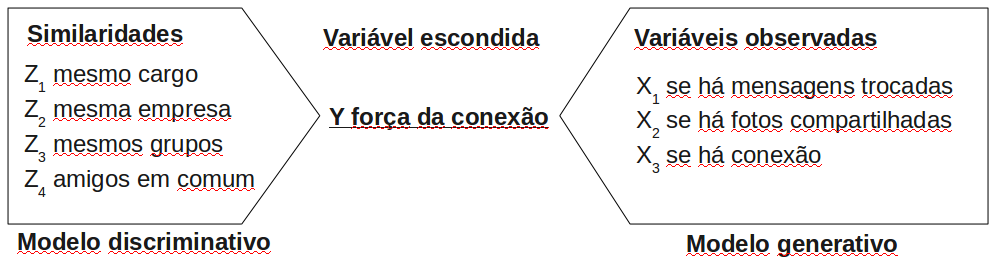
\includegraphics[width=\textwidth]{imgs/modeloXiang.png}
	\caption{modelo da força da conexão como variável escondida \citep{Xiang2010}.}
	\label{fig:xiang}
\end{figure}

No primeiro momento, para uma amostragem dos atores, são observadas as variáveis
de interação, como se há troca de mensagens, fotos ou se foi estabelecido uma
conexão entre os atores; são também coletadas as similaridades, como a presença
nos mesmos grupos, a existência de amigos em comum e a equivalência de cargos e
funções. No segundo, a força da conexão é inferida como variável latente que é
dependente da similaridade e da qual dependem as variáveis de interação
observadas. Os pesos dessas dependências são ajustados iterativamente de forma a
maximizar a probabilidade da ocorrência das variáveis observadas. Uma vez
ajustados os pesos, a partir da similaridade de dois atores quaisquer será
possível calcular a força de sua conexão. Essa combinação de modelo discriminativo e
generativo possibilita a inferência não supervisionada da força da conexão, o que
é um ponto positivo para esta abordagem, porém ela subestima outros fatores
igualmente importantes.

A similaridade é apenas uma das possíveis componentes da força da conexão,
propriedade conhecida como homofilia. Para um entendimento de um processo geral
de mensuração da rede digital, precisamos remontar a um dos trabalhos fundantes
da análise de redes sociais onde \citeauthor{Granovetter1973} lança, pela
primeira vez, a hipótese:

	\begin{quote}{\citep{Granovetter1973}}
	\emph{A força da conexão [entre dois atores] é uma combinação
	(provavelmente linear) da quantidade de tempo, intensidade emocional,
	intimidade (confidência mútua) e serviços recíprocos que a
	caracterizam.} 
	\end{quote}

\citeauthor{Granovetter1973} também separa indicadores de pescritores,
indicadores são componentes de fato da força da conexão, enquanto que
prescritores são contigências contextuais que influenciam, mas não são
componentes. Dentre os prescritores está a homofilia, o que quer dizer que a
similaridade entre os atores tem, de fato, alguma influencia sobre a conexão, mas
é a intensidade, duração, intimidade e reciprocidade da interação que indicam a
sua força. Dessas quatro dimensões iniciais (tempo, intensidade, intimidade,
reciprocidade), acrescentaram-se nove outras no decorrer de três décadas de
pesquisa. Na \tabref{tab:resumao} temos um apanhado dos indicadores propostos na
literatura.

Em \citet{Gilbert2009} encontramos uma análise da composição desses indicadores
na força da conexão. Através de um modelo discriminativo os autores encontram a
correlação linear entre 74 variáveis em cima das interações coletadas no site de
relacionamento Facebook e a força da conexão coletada através de questionário
com uma amostra de 32 indivíduos. Sua análise leva em consideração sete indicadores
de força, separando as variáveis em dimensões do tipo intensidade, intimidade,
duração, reciprocidade, estrutural, emocional, similaridade. É interessante
notar que duas dimensões escolhidas são consideradas como prescitoras da força e
não indicadoras, que são a estrutura e a similaridade. Sobre similaridade já
falamos, já as variáveis estruturais referem-se a padrões da rede como a
transitividade, i.e., amigo de amigo seu tem maior chance de ser seu amigo
também.

Os resultados mostram uma partição da força por dimensão que pode ser vista na
\figref{fig:forca}. As dimensões de intimidade, intensidade e duração são as três
maiores componentes da força, como previsto por \citeauthor{Granovetter1973}. As
variáveis de estrutura, sozinhas, são as que menos utilidade tem para a previsão
da força, porém quando analisada em par com outras dimensões demonstram alto de
grau de interação. Nas palavras dos autores:

	\begin{quote}{\citep{Gilbert2009}}
	\emph{A dimensão estrutural possui um papel menor como fator linear.
	Entretanto, ela possui um papel regulador importante através dessas interações
	[com as outras dimensões]. Uma forma de interpretar este resultado é que
	interações individuais importam, porém elas são filtradas através do
	clique\footnotemark de amigos antes de impactar a força da
	relação.}
	\end{quote}

\footnotetext{clique pode ser traduzido como grupo de amigos com interesses
similares e que são vistos por outros como exclusivistas; panelinha.}

\begin{figure}[h!]
  \centering
    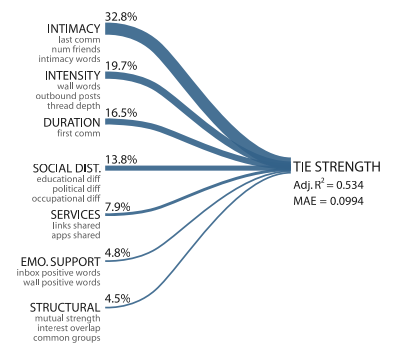
\includegraphics[width=0.7\textwidth]{imgs/composicao-forca.png}
  	\caption{Poder preditivo das sete dimensões da força da conexão
  	\citep{Gilbert2009}}
    \label{fig:forca}
\end{figure}

Esse resultado confirma o papel prescritivo das variáveis estruturais. Não
obstante os resultados, o método de \citet{Gilbert2009} possui restrições quanto
a utilidade em nosso cenário digital. Em primeiro lugar, sua abordagem
supervisionada não escala com a rede e não há estudo sobre o erro induzido pela
amostragem. Em segundo lugar, o tipo de conexão não é direcionado, isto é, ambos
atores conferem o mesmo valor para a relação. Essa simplificação é nociva para o
nosso objetivo de análise de influência, já que a assimetria de influência é
bastante comum, por exemplo, um aluno pode ter grande consideração por um
professor, mas o inverso em pé de igualdade raramente é verdade.

\begin{table} [htbp]
	\setlength{\arrayrulewidth}{2\arrayrulewidth}  % espessura da  linha
	\setlength{\belowcaptionskip}{10pt}  % espaço entre caption e tabela
	\caption{Sumário dos componentes da força da conexão
	\citep{Petroczi2006}} \centering   % tabela centralizada
	\begin{tabular}{| p{4cm} | p{8cm} |}
	\hline
	\textbf{Dimensão} & \textbf{Referências} \\ \hline\hline
	Frequência & \citet{Benassi1999, Blumstein1988, Granovetter1995,
	Marsden1984, MATHEWS1998, Mitchell1987, Perlman1987} \\\hline
	Intimidade & \citet{Blumstein1988, Marsden1984, MATHEWS1998, Mitchell1987,
	Perlman1987}\\\hline 
	Investimento voluntário na relação & \citet{Blumstein1988, Perlman1987}\\\hline
	Aconselhamento dado e recebido & \citet{MATHEWS1998}\\\hline 
	Desejo de companhia & \citet{Blumstein1988, Perlman1987}\\\hline 
	Multiplicade dos contextos em que há interação & \citet{Blumstein1988,
	Granovetter1973, Marsden1984, Perlman1987}\\\hline 
	Duração & \citet{Blumstein1988, Granovetter1973, Marsden1984,
	Perlman1987}\\\hline 
	Reciprocidade & \citet{Blumstein1988, Friedkin1980, Granovetter1973,
	MATHEWS1998, Perlman1987}\\\hline 
	Suporte	emocional (intensidade) & \citet{Blumstein1988, Granovetter1973,
	Mitchell1987, Perlman1987, Wellman1982, Wellman1990}\\\hline
	Confiança & \citet{Granovetter1973, Marsden1984, MATHEWS1998}\\\hline
	Sociabilidade & \citet{Mitchell1987}\\
	\hline
	\end{tabular}
	\label{tab:resumao}
\end{table}

Isso nos leva a reflexão de que, para análise de influência, a utilização de
todas as dimensões da força da conexão pode ser muito restritiva. Uma delas, como
no exemplo já citado, é a dimensão de reciprocidade: um ator com prestígio exerce
grande influência sobre seus admiradores, mas cada admirador individualmente não
consegue exercer influência de igual intensidade sobre ele. Outro exemplo são os
indíviduos de fronteira, que se conectam à periferia de dois grupos; as suas
conexões são fracas, mas exerce grande influência na transferência de
conhecimento entre os grupos. Daí temos que apesar da noção de força de
Granovetter está relacionada com a influência, ela não é condição necessária
\citep{Brown2007}.

Finalmente, nenhuma das soluções estudadas considera a evolução da rede no
tempo. Nesse aspecto algumas pesquisas utilizam ``fotografias'' na rede em
momentos diferentes ou agregações das interações por período. A partir daí
utiliza-se modelos probabilísticos \citep{Sarkar2005}, meta-grupos
\citep{Berger-Wolf2006} ou modelos provenientes da psicologia comportamental e da
administração \citep{Brelger2004}. Nenhum deles, entretanto, é combinado com
a teoria da força das conexões para permitir sua aplicação em processos de
mensuração de redes sociais digitais.

A partir de então sugerimos alguns critérios para as ferramentas de mineração
que serão usadas no processo de análise de influência:

\begin{enumerate}
  \item Deve ser não supervisionada para aumentar a chance de escalar com o
  tamanho da rede;
  \item Deve considerar a força das relações na maior quantidade possível de seu
  espectro de componentes. Por tanto, a representação resultante não deve ser
  binária;
  \item Deve também levar em consideração aspectos estruturais da rede como
  transitividade e \emph{brokerage};
  \item Deve ser longitudinal, isto é, incorporar o elemento tempo na análise,
 levando em conta a formação e dissolução de relações, entrada e saída de
 atores;
\end{enumerate}

Uma vez escolhida as ferramentas de mensuração e análise, devemos agora avançar
para o passo seguinte e selecionar quais dados serão usados e se eles são
válidos.

